\section{The Dataset}

\begin{frame}{Problem Setting}
	\begin{block}{}
		We define the multimodal input space as the Cartesian product of $P$ modality-specific input spaces:
		\[
		\mathcal{X} = \prod_{p=1}^{P} \mathcal{X}^{(p)},
		\]
		where each modality $\mathcal{X}^{(p)}$ may represent data from distinct sources.
	\end{block}
	
\end{frame}



\begin{frame}{Toadstool 2 Dataset}
\begin{block}{}
The dataset consists of video, sensor, and demographic data collected from 10 participants playing a Super Mario Bros.
\end{block}

\vspace{-0.5em}

		\begin{columns}[T] % Top alignment
		\begin{column}{0.5\textwidth}
			\begin{center}
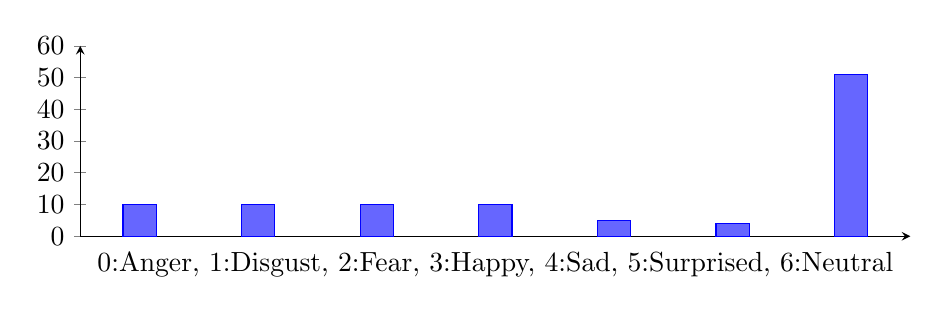
\begin{tikzpicture}
	\begin{axis}[
		width=\textwidth,
		height=4cm,
		ybar,
		bar width=12pt,
		axis x line=bottom,
		axis y line=left,
		xlabel={0:Anger, 1:Disgust, 2:Fear, 3:Happy, 4:Sad, 5:Surprised, 6:Neutral},
		xtick=\empty,               % no individual ticks on x
		ytick={0,10,20,30,40,50,60},
		ymin=0, ymax=60,
		xmin=-0.5, xmax=6.5,        % margin for first/last bar
		]
		\addplot+[fill=blue!60] coordinates {
			(0,10) (1,10) (2,10) (3,10) (4,5) (5,4) (6,51)
		};
	\end{axis}
\end{tikzpicture}


			\end{center}
			
		\end{column}
		\begin{column}{0.5\textwidth}
		\centering
		\small
		\begin{tabular}{lcc}
		\toprule
		\textbf{Signal} & \textbf{Rate (Hz)} & \textbf{Channels} \\
		\midrule
		BVP  & 64 & 1      \\
		ACC  & 32 & 3 		\\
		EDA  & 4  & 1      \\
		HR   & 1  & 1      \\
		\bottomrule
		\end{tabular}
		
		\begin{block}{}
			20 970 sensor‐only samples (4 s windows)
		\end{block}

		\end{column}
		
	\end{columns}
\end{frame}


\begin{frame}[t]{Problem Setting}

	\begin{block}{}
		Let $\{\boldsymbol{x}^{(i)}, y^(i)\}_{i=1}^{N}$ be the train dataset, with $\boldsymbol{x}^{(i)}\in\mathcal{X}$ and $y \in \{\}\}$.  Each sequence is
		\[
		x^{(i)}
		=\bigl[x^{(i)}_{t_{1}},\dots,x^{(i)}_{t_{n_i}}\bigr],
		\quad t_k = \tfrac{k}{64}\,\mathrm{s},\;k=1,\dots,n_i.
		\]
		For modality $p$ at lower native rate,
		\[
		x^{(i,p)}_{t_k} =
		\begin{cases}
			\text{observed}, & t_k\in T^{(p)},\\
			\mathrm{NaN},    & \text{otherwise},
		\end{cases}
		\]
		where $T^{(p)}$ are the true sampling instants of modality $p$.
	\end{block}
\end{frame}
